%\documentclass{article} % For LaTeX2e
\documentclass[conference,10pt]{IEEEtran}
%\usepackage{nips14submit_e,times}

\usepackage[sc]{mathpazo}
%\linespread{1.05}         % Palatino needs more leading (space between lines)
\usepackage[T1]{fontenc}

\usepackage{url}
%\documentstyle[nips13submit_09,times,art10]{article} % For LaTeX 2.09

\usepackage{hyperref}
\usepackage[usenames,dvipsnames]{color}
\definecolor{orange}{rgb}{0.8,0.4,0}
\definecolor{mylink}{RGB}{18,68,115}
\definecolor{darkgreen}{rgb}{0.3,0.6,0.3}

\usepackage{graphicx}
%\usepackage[footnotesize]{caption}
\usepackage[numbers,sort&compress]{natbib}

\hypersetup{letterpaper,bookmarksopen,bookmarksnumbered,
pdfpagemode=UseOutlines,
colorlinks=true,
linkcolor=mylink,
anchorcolor=blue,
citecolor=mylink,
filecolor=blue,
menucolor=blue,
urlcolor=mylink,
}
%\usepackage{multicol}
 
% Labels in IEEE format
% Equation
\newcommand{\eref}[1]{Eq.(\ref{#1})}
% Figure
\newcommand{\figref}[1]{Fig.\ref{#1}}

\usepackage{ifthen}

\newboolean{include-notes}
\setboolean{include-notes}{true}
% http://en.wikibooks.org/wiki/LaTeX/Colors
\newcommand{\ssnote}[1]{\ifthenelse{\boolean{include-notes}}%
 {\textcolor{orange}{\textbf{SS: #1}}}{}}
\newcommand{\adnote}[1]{\ifthenelse{\boolean{include-notes}}%
 {\textcolor{LimeGreen}{\textbf{AD: #1}}}{}}

\usepackage[font=footnotesize]{caption}
\usepackage{subfigure}

\title{\Large Real-time Surface Reconstruction on a Mobile Device \\
using Chunked Truncated Signed Distance Fields}


\newcommand{\fix}{\marginpar{FIX}}
\newcommand{\new}{\marginpar{NEW}}

%\nipsfinalcopy % Uncomment for camera-ready version
\usepackage{amsmath,amssymb,amsthm}
\begin{document}

\author
{
	Matthew Klingensmith \\
	Carnegie Mellon Robotics Institute\\
	\texttt{mklingen@andrew.cmu.edu}
	\and
	Ivan Dryanovski \\
	City College of New York\\
	\texttt{ivan.dryanovski@gmail.com}
}


\maketitle

\begin{figure}[t]
  \centering
    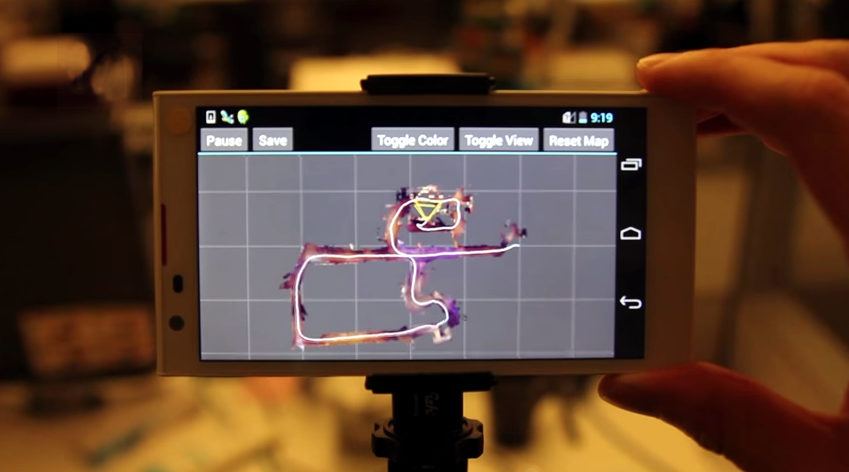
\includegraphics[width=1.0\columnwidth]{img/mapdevice}
      \caption{Our algorithm recording a map of an office building floor on a mobile
  device in real time, at a resolution of 3cm.}
  \label{fig:map_device}
\end{figure}


\begin{abstract}
Abstract here
\end{abstract}

\section{Introduction}
% \begin{itemize}
%     \item We want to do large-scale 3D reconstruction from depth data with only
%     limited hardware.
%     \item This is attractive for many use cases where all one wants to do is
%     make a rough mesh of an area. The real-time aspect allows the user to see
%     the accuracy of the reconstruction easily. This is also attractive for small
%     mobile robots (such as quad-copters) with limited onboard compute power.
%     \item We have access to VIO, and so don't need to do pose estimation
%     \item Existing techniques are not sufficient for the amount of compute power
%     we have
%     \item We want to be careful about maintaining probabalistically accurate
%     data and not throwing it away/compressing it.
%     \item It's important to keep track of the noise model of the sensor to deal
%     with noise, distortion and missing data.
%     \item We want to use the TSDF over occupancy grids \cite{Elfes1989} or
%     octomaps \cite{Wurm2010}, because the TSDF is much better at maintaining
%     surface information, and occupancy information can easily be extracted from
%     it.
%     \item We also want to use the color camera, but don't want to make a
%     photometrically accurate model due to our limited compute power.
% \end{itemize}

Mobile devices are beginning to offer a wide range of sensors normally found on
robots: gyroscopes, accelerometers, compasses, GPS units, and high resolution
sensors are now common place in average market phones. Recently, mobile phone
manufacturers have expressed interest in using depth sensors in mobile devices;
this opens up interesting possibilities for 3D reconstruction, mapping,
and object recognition on such devices that were previously unavailable. Mobile
devices with depth sensors also provide an attractive, light-weight, integrated
platform for small mobile robots.

We are interested in the problem of real-time 3D reconstruction. The task is to
extract the true 3D geometry and color of a real scene from a sequence of noisy
sensor readings. Solutions to this problem are useful for mobile robot navigation,
indoor localization, mapping, and object scanning. The problem is ill-posed,
since it requires localization as well as mapping (and hence is a variant of
the SLAM problem.)

Real-time 3D reconstruction remains challenging on mobile devices. Compared to
full-sized machines, mobile devices have severely limited processing power,
memory requirements, and graphics capabilities. Further, the depth sensors
available on these devices are much more limited than their full-sized
counterparts; they are typically lower resolution, have slower refresh rates,
and have much more undesirable nonlinear distortion and noise.

Previous work on high quality real-time 3D reconstruction has focused on much
more capable and high-powered computing platforms with much more accurate
sensing, and is therefore not well suited for low-powered mobile devices.

In this work, we propose a novel algorithm for efficient real-time 3D
reconstruction on mobile devices with onboard depth sensors. We show that even
with a low-powered mobile device with severe limitations on memory usage, 
processing power, and graphics capabilities, relatively high-quality,
large-scale real-time 3D reconstruction is feasible.

\section{Related Work}
% \begin{itemize}
%     \item Real-time mapping solutions started with occupancy grids
%     \cite{Elfes1989}. But implemented in a naive way, these are too memory
%     intensive for our purposes. They are also bad at surface reconstruction.
%     \item More recent work in occupancy grid mapping reduces their memory
%     footprint by introducing an octree structure \cite{Wurm2010}. However,
%     octree structures have a hefty lookup time for each access, read, or write.
%     They also have poor cache performance during iteration.
%     \item \cite{Curless1996} introduced the TSDF as an efficient, accurate way
%     of reconstructing surfaces from many registered depth images. These are more
%     desirable for surface reconstruction than occupancy grids, because they
%     maintain local structure (inside vs. outside).
%     \item \cite{Newcombe}, introduced a method (Kinect Fusion) of creating and
%     registering TSDF volumes to depth images in real-time using ICP-like alignment of scans.
%     Making heavy use of GPU computing, Kinect fusion is able to generate and
%     display extremely high-quality reconstructions in a small area (due to
%     using a fixed size volume for reconstruction). 
%     \item Attempting to increase the size of Kinect Fusion reconstructions and
%     reduce drift, Kintinuous \cite{Whelan2013} keeps a running window of the
%     scene that gets integrated into a TSDF. Parts of the scene outside the
%     window are turned into a mesh with simple greedy triangulation. While this
%     allows them to make larger reconstructions than Kinect Fusion, they lose
%     distance field data as they move around the scene -- data which might still
%     be useful in its uncompressed form. We want to do large-scale reconstruction
%     \emph{without} compressing volumetric data into a surface representation
%     first.
%     \item Like \cite{Whelan2013}, \cite{Bylow2013} use the volume structure
%     directly to store colors. We copy the method of \cite{Bylow2013} to colorize
%     our meshes due to the simplicity and speed of the method.
% \end{itemize}
Real-time mapping has long been a research topic in robotics and computer
vision. One of the simplest means of 3D reconstruction is to simply store a
\emph{Point Cloud} of the scene. This is done by projecting depth images into
the scene as points, and then aligning point clouds to the existing scene.
While simple, point clouds fail to capture local scene structure, are highly
redundant, noisy, and memory intensive. Additionally, point clouds fail to
capture \emph{negative} information about the scene : \emph{i.e}, determining
which parts of the scene are empty. This information is crucial in situations
where the sensor is noisy, or has large patches of missing data
\cite{Klingensmith2014}.

Elfes \cite{Elfes1989} introduced the concept of \emph{Occupancy Grid
Mapping}, which divides the world into a 2D grid of axis-aligned cells
(\emph{i.e} Voxels), each of which contains an occupancy probability. Occupancy
grids provide a principled alternative to simple point clouds. They preserve local
structure, and gracefully handle redundant and missing data.
Unfortunately, occupancy grids are prohibitively memory intensive in 3D, since
the amount of memory needed to store the grid increases with the cube of distance 
traveled by the sensor. While more robust than point clouds, occupancy grids
suffer from aliasing, and lack information about surface normals and the
interior/exterior of obstacles.

Attempts to extend occupancy grid maps to 3D have sometimes relied on octrees.
Rather than storing a fixed-resolution grid, octrees store occupancy data in a
spatially organized tree. In typical scenes, octrees reduce the required memory
over occupancy grids by orders of magnitude. Octomap \cite{Wurm2010} is a
popular example of the octree paradigm. However, octrees containing only
occupancy probability suffer from many of the same problems as occupancy grids:
they lack information about the interior and exterior of objects, and suffer
from aliasing. Further, octrees suffer from logarithmic reading, writing, and
iteration times, and have very poor memory locality characteristics.

Curless \cite{Curless1996} introduced an alternative to occupancy grids for 3D
reconstruction which, instead of storing the occupancy probability for each
voxel, stores an approximation of the signed distance field of the scene. The signed distance
field is a mapping from $\mathbf{R}^3$ to $\mathbf{R}$ which represents the
distance to the nearest surface. The SDF is negative inside obstacles, and
positive outside obstacles. The surface is given implicitly as all points in
space where the value of the SDF is zero. The structure introduced in
\cite{Curless1996} only maintains the distance function within a small distance 
(called the \emph{truncation distance}) from observed surfaces, and thus is called the
Truncated Signed Distance Field (TSDF).  While using more memory than occupancy
grids, the TSDF is much more informative for surface reconstruction, as the
implicit surface normals can be extracted from the gradient of the function,
allowing for a higher quality reconstruction.

The \emph{Kinect Fusion} \cite{Newcombe} algorithm uses a TSDF to
simultanesously extract the pose of a moving depth camera and the geometry of a scene in real-time. Kinect
Fusion solves the real-time 3D reconstruction problem by using incremental
estimates of the TSDF to inform the pose of the camera. Making heavy use of the
GPU for raycasting and rendering, Kinect Fusion is capable of creating extremely
high-quality, high-resolution surface reconstructions within a small area.
However, like occupancy grid mapping, the algorithm relies on a single
fixed-size 3D grid of voxels, and thus is not suitable for reconstructing very
large scenes. Fusion also suffers from pose drift as small localization errors
accumulate.

The \emph{Kintinuous} \cite{Whelan2013} algorithm extends Kinect Fusion to
larger scenes by storing only a time-limited moving window of the TSDF. As the camera
moves outside of the window, areas which are no longer visible are turned into a
triangular mesh. Like Fusion, Kintinuous relies on very high-performance GPU
computing to create its reconstruction.  By prematurely turning the TSDF into an
explicit surface mesh, Kintinuous throws away past data -- and thus the user
cannot return to an area that was previously explored and update the TSDF there.

Our approach uses a TSDF as in
\cite{Curless1996,Newcombe,Whelan2013,Bylow2013}, to store an
estimate of the signed distance field of the scene. Unlike Kinect Fusion, and like Kintinuous,
we store a dynamic representation of the TSDF which grows in size as the sensor
travels through space. Unlike Kintinuous, we do not prematurely throw away
distance function data by converting it into a mesh -- instead, we turn small
areas of the scene into meshes for the purpose of rendering, and preserve the
underlying distance field data. In this way, we extend the TSDF surface
reconstruction paradigm to very large scenes when only very limited compute
power is available.

\section{Approach} 
% \begin{itemize}
%     \item We start by getting an accurate probablistic model of the depth error
%     on the sensor by training a quadratic model of the depth and noise per
%     pixel. Depth images are compensated by this model before being passed into
%     our system.
%     \item We get pose by monocular visual-intertial odometry, rather than by
%     directly estimating pose from the depth image.
%     \item Depth comes in at 3-5Hz, as does RGB, but never at the same time.
%     \item Explain the TSDF
%     \item We represent the world as a collection of fixed size 16x16x16
%     \emph{Meta-Voxels} or \emph{Chunks}, aligned next to each other. Chunks are
%     allocated only when rays from the sensor would cause them to be updated.
%     They are garbage collected whenever there is no voxel with no weight in it.
%     \item To update a chunk with depth data, we can do one of two things:
%     \emph{Raycasting}, or \emph{Voxel Projection}. In the raycasting case, we
%     efficiently march rays through voxels in each updated TSDF volume, and
%     update the signed distance and weight there. In the voxel projection case,
%     we project the center of each voxel onto the image, and according to the
%     distance from the center of the voxel as compared with the depth from the
%     sensor, we either add weight to it, carve it, or do nothing to it.
%     \item Raycasting is O(number of rays), while Voxel Projection is O(number
%     of voxels). Voxel projection is an aliased approximation of raycasting. 
%     \item To do color, we project the points along the ray we are updating onto
%     the color image. We then update a separate \emph{Color Chunk} with data from
%     the RGB image.
%     \item We use a dynamic trunction distance based on the sensor model.
%     \item Rendering is handled by incrementally creating meshes of the updated
%     chunks using Marching Cubes. Chunks are frustum culled based on the frustum
%     of the renderer's camera, and only those which are near the camera and
%     inside its frustum are rendered. Faraway chunks are rendered as boxes. This
%     allows us to very efficiently render huge areas using only the fixed
%     function pipeline -- an important feature for devices with limited graphics
%     capability.
% \end{itemize}
\subsection{Depth Data and Noise Model}
We begin by considering the data from the device. We will assume that the device
has a depth sensor attached. The depth sensor produces a depth image, which is
a discrete map containing sensed distances from the scene to the image plane.

Consider an ideal pinhole camera model of the depth sensor. We can cast a ray
from the sensor origin through the image plane to surfaces in the world. The
length of that ray is the resulting depth at that point in the image plane. Call
the point on the image plane that the ray intersects $u$. The length of the ray
through $u$ to the scene is given by $z_u$. 

The depth image may be corrupted by noise, feature nonlinear distortions, and
have large segments of missing data. Our noise model of the sensor will consider
Gaussian noise on the depth, and per-pixel quadratic distortion. Call the depth
 measurement at $u$ the random variable $D_u$. Then,
 
 $$ D_u = z_u + a_u{z_u}^2 + b_u z_u + c_u + \epsilon(z_u)$$
 
 \noindent where $a_u, b_u, c_u$ are coefficients of a quadratic depth
 distortion model, and $\epsilon(z_u)$ is a random variable drawn from the
 parametric gaussin distribution function $\mathcal{N}(z_u, \sigma_{z_u})$. 
 That is, the distribution is mean-centered on $z_u$, and has a depth-dependant
 standard deviation $\sigma_{z_u}$.
 
 We found that, on our devices, the nonlinear distortion was very severe. At a
distance of 3 meters, the reading could be distorted by as much as 30
centimeters. To get an accurate reconstruction of the world, it is critical to
correct for this distortion.
 
 To train the distortion and noise model, we first calibrate the sensor with the
 use of a checkerboard calibration target. Images of the target are taken at
 multiple distances and angles from the camera. We fit an ideal plane to the
 target to determine what the true distance should be at each pixel. Then, we
perform quadratic regression on the depth readings against the predicted
readings from the plane to find the per-pixel distortion coefficients. The
coefficients are stored in a database for later use.

The function $\sigma_{z_u}$ is computed in a similar way, by computing a
histogram of standard deviations of the depth readings, and then performing
quadratic regression on the result. A single function $\sigma_{z_u}$ is used for
the entire image, unlike the distortion model which is computed on a per-pixel
basis.

Finally, we preprocess all depth images from the device by inverting the
distortion model to get an estimate of the true depth at each point on the
image plane.

\textbf{TODO: DESCRIBE THE ABOVE PROCEDURE IN MORE DETAIL. CITE IVAN'S WORK.
FIGURES OF DATA? FIGURES OF THE PLANE?}

\subsection{Pose Estimation}
We will assume we have black-box pose estimation of the sensor from a seperate
system. Specifically, in our experiments, pose data is estimated from an
embedded visual-intertial odometry system that fuses data from a wide-angle camera, an
intertial measurement unit, and a gyroscope at 60 Hz. \textbf{TODO: DESCRIBE
THIS IN MORE DETAIL AND CITE SOME VIO RESEARCH}

Unlike \textit{Kinect Fusion} \cite{Newcombe} and \textit{Kintinuous}
\cite{Whelan2013}, Our approach makes no attempt to estimate the pose of the
sensor directly from depth data. Instead, we use depth data only for surface
reconstruction.

Call the global pose estimate of the sensor at time $t$,  ${H_{s}}^t$.
Additionally, assume we have apriori extrinsic pose estimates for the color
sensor ${H_{c}}^t$ and the depth sensor ${H_{d}}^t$. We will assume that pose
estimation, depth sensing, and color sensing are asynchronously executed, so we
may not have all three measurements at a given time.

To deal with asynchronous sensing and pose estimation, we linearly interpolate
poses over time to determine the pose of a given sensor at any given time.
\textbf{TODO: DESCRIBE THIS BIT IN DETAIL.}.

\subsection{The Signed Distance Function}
We model the world as a volumetric function $\Phi(x) : \mathbf{R}^3 \to
\mathbf{R}$, where, for every 3D point in the world, we have its distance to the
nearest surface of an object. Inside objects, the value of $\Phi$ is negative.
Outside objects, the value of $\Phi$ is positive, and on the surface, it is
zero.

 We will assume that $\Phi$ is static (\textit{i.e} it contains no moving
 objects aside from the sensor itself). We want to estimate the value of $\Phi$
 from the depth data and sensor poses over time.

Consider the geometry of the ideal depth sensor. Rays emenate from the sensor
origin to the scene. Call the origin of the ray $o$, and the endpoint of the ray
$x$. The direction of the ray is given by $r = \frac{o - x}{\|o - x\|}$.

The endpoint of each ray represents a point on the surface. So if the sensor is
perfect, we know that the signed distance function $\Phi(x) = 0$ at that point. 

But what else does the ray tell us? All the points in space along the ray from
the sensor origin up to the endpoint must be outside of any surface (or else the
ray would have been occluded by a a surface). Assuming objects have non-zero
thickness, some part of the space along the ray beyond the endpoint should be
inside an object. That is:

$$ \Phi(x - ur) 
     \begin{cases}
     > 0 & \text{if } u > 0 \\
     < 0 & \text{if } u < 0 \\
     0 & \text{if } u = 0
     \end{cases}
     $$

Further, very near the surface of the object, the signed distance function can
be approximated by the distance along the ray to the endpoint of the ray. This
is because we know that there is at least one point of the surface, namely the
endpoint of the ray. Near $x$, the signed distance function scales with the
distance to $x$. So:

$$ \Phi(x - ur) \approx u $$

\noindent Whenever $u \approx 0$. This leads us to the Truncated Signed Distance
Function (TSDF) \cite{Curless1996}. The TSDF is an approximation of the Signed
Distance Function which stores distances to the surface within a small truncation distance,
$\tau$. That is:

$$ \Phi_{\tau}(x) \begin{cases}
	 = \Phi(x) & \text{if } |\Phi(x)| \leq \tau \\
	 \text{undefined} & \text{otherwise}
	 \end{cases}
$$

Following \cite{Curless1996}, to update the TSDF with a particular sensor
measurement, we integrate along the ray from $u = -\tau$ to $\tau$, and take the
running average over time. To do this, we introduce a weighting function $w :
\mathbf{R}^3 \to [0, 1]$ that represents our confidence in the estimate of the
TSDF.

\begin{align*}
\Phi_{\tau}(x - ur) \gets w_u\ \Phi_{\tau}(x - ur) + (1 - w_u) \\
%
w_u \gets w_u+ \alpha 
\end{align*}

\noindent Where  $w_u = w(x - ur)$, and $\alpha \in [0, 1]$ is a weighting
parameter.


\section{Results}
\begin{itemize}
    \item We are able to reconstruct very large areas at a relatively high (3
    cm) resolution on a mobile device.
    \item We have a limited memory footprint, and each frame is processed on
    the CPU in less than 150 ms.
    \item Show comparisons of different parts of our technique being used
    (voxel carving vs. not, projection vs. raycasting) in terms of speed, memory
    efficiency, and so on. Also show pictures.
    \item Show the difference between merely doing online odometry vs. offline
    bundle adjustment
\end{itemize}

\section{Discussion and Future Work}
\begin{itemize}
    \item If we're keeping around the volumetric information, what does that buy
    us? Can it help us with loop closure?
    \item These techniques can be used outside of the mobile context to speed
    things up.
    \item We gain a lot by using decoupled pose, but there needs to be a way to
    incorporate the VIO pose with dense alignment (like they do in Kintinuous).
\end{itemize}

\section{Acknowledgements}
\begin{itemize}
    \item Thank project Tango, ATAP, the team.
\end{itemize}

\bibliographystyle{plain}
% argument is your BibTeX string definitions and bibliography database(s)
\bibliography{densemapping, ./densemapping} 
\end{document}